% Editable reconstruction; interpretation recorded in root.json.
% Shared standalone design for the editable figure reconstructions.
\documentclass[tikz,border=5pt,10pt]{standalone}
\usepackage[T1]{fontenc}
\usepackage[utf8]{inputenc}
\usepackage{newpxtext,newpxmath}
\usepackage[scaled=.94]{sourcesanspro}
\usepackage{pgfplots}
\pgfplotsset{compat=1.18}
\usetikzlibrary{arrows.meta,calc,positioning,decorations.pathreplacing,
  decorations.markings,patterns,matrix,shapes.geometric,fit,backgrounds,
  intersections,angles,quotes}
\definecolor{ink}{HTML}{203746}
\definecolor{accent}{HTML}{146C78}
\definecolor{muted}{HTML}{667780}
\definecolor{signalred}{HTML}{B94B44}
\color{ink}
\tikzset{>=Latex,line width=.8pt,
  every node/.style={font=\small},
  axis/.style={->,draw=muted,line width=.5pt},
  guide/.style={draw=muted,dashed,line width=.45pt},
  curve/.style={draw=accent,line width=1pt},
  marker/.style={circle,fill=accent,inner sep=1.5pt},
  labelbox/.style={fill=white,inner sep=2pt}}

\begin{document}

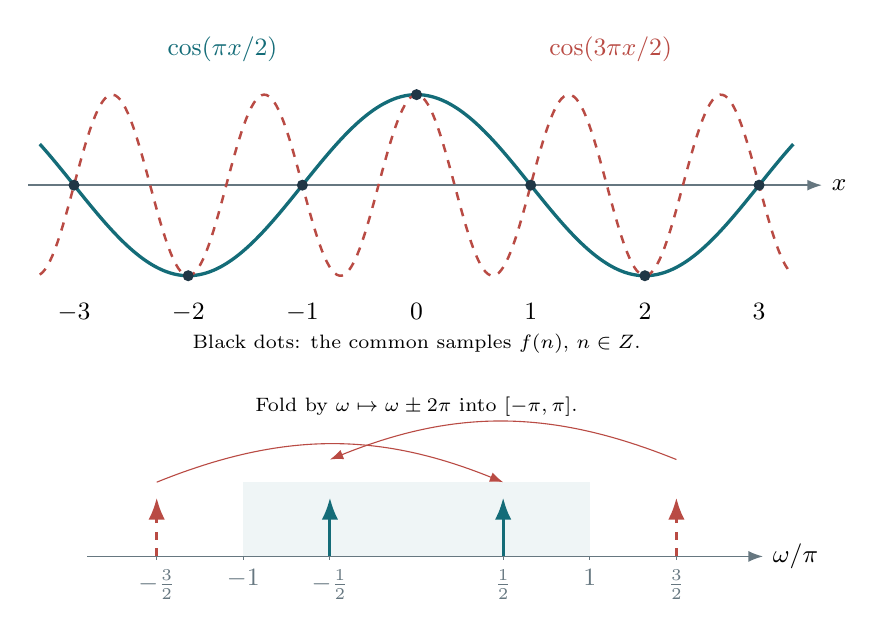
\begin{tikzpicture}[x=1.45cm,y=1.15cm]
\draw[axis] (-3.4,0)--(3.55,0) node[right] {$x$};
\draw[accent,line width=1.2pt,domain=-3.3:3.3,samples=250] plot (\x,{cos(90*\x)});
\draw[signalred,dashed,line width=.9pt,domain=-3.3:3.3,samples=300] plot (\x,{cos(270*\x)});
\foreach \n in {-3,-2,-1,0,1,2,3}{\fill[ink] (\n,{cos(90*\n)}) circle(2pt);\node[below] at (\n,-1.2) {$\n$};}
\node[accent] at (-1.7,1.5) {$\cos(\pi x/2)$};\node[signalred] at (1.7,1.5) {$\cos(3\pi x/2)$};
\node[font=\scriptsize] at (0,-1.75) {Black dots: the common samples $f(n)$, $n\in\mathbb Z$.};
\begin{scope}[shift={(0,-4.1)},x=2.2cm]
\fill[accent!7] (-1,0) rectangle (1,.82);
\draw[axis] (-1.9,0)--(2,0) node[right] {$\omega/\pi$};
\foreach \x/\lab in {-1.5/-\frac32,-1/-1,-.5/-\frac12,.5/\frac12,1/1,1.5/\frac32}{\draw[muted] (\x,0)--(\x,-.04) node[below] {$\lab$};}
\foreach \x in {-.5,.5}{\draw[->,accent,line width=1.1pt] (\x,0)--(\x,.65);}
\foreach \x in {-1.5,1.5}{\draw[->,signalred,dashed,line width=1.1pt] (\x,0)--(\x,.65);}
\draw[->,signalred] (-1.5,.82) to[bend left=22] (.5,.82);
\draw[->,signalred] (1.5,1.07) to[bend right=22] (-.5,1.07);
\node[font=\scriptsize] at (0,1.65) {Fold by $\omega\mapsto\omega\pm2\pi$ into $[-\pi,\pi]$.};
\end{scope}
\end{tikzpicture}
\end{document}
